\subsection{UCS (Uniform Cost Search)}\lezione{Lezione 5}{14/10/2024}
Nella presentazione di BFS e DFS, abbiamo sempre ipotizzato di dover risolvere problemi di Fattibilità (paragrafo \ref{def:fattibilità}),
per cui i 2 algoritmi hanno dovuto solo esplorare il grafo fino a generare un nodo obiettivo del problema.
Per risolvere il problema di Ottimizzazione, invece, dovremo utilizzare l'approccio conservativo della BFS per progettare 
un algoritmo che trovi sempre il percorso ottimo.\\

\paragraph{Cost To Go Function. }
Per descrivere l'implementazione della UCS è necesasario innanzitutto definire la \textit{Cost-to-Go Function} $g(V)$.
Dato un vertice $V$, $g(V)$ è il costo complessivo per arrivare dallo stato $A$ allo stato $V$ tramite un percorso $p$.

\subsubsection{Algoritmo (Ad alto livello)}
Inizialmente si aggiunge alla Frontiera il nodo di Partenza $A$ e dopodichè
\begin{itemize}
    \item Si calcolano per ogni nodo della frontiera il $g(V)$
    \item Si seleziona il nodo da espandere con $g(V)$ più piccolo
    \item Ci si ferma solo quando \textbf{espandiamo} un nodo Goal
\end{itemize}

\newpage

\subsubsection{Ottimalità di UCS}
Si può dimostrare che UCS non solo è \textbf{corretto} e \textbf{completo} e che seleziona il percorso \textbf{ottimo}, ma che
\textit{"Ogni volta che UCS seleziona per la prima volta un nodo per l'espansione, il percorso che porta ha quel nodo ha costo minimo"}

\paragraph{Ipotesi. }
\begin{enumerate}
    \item UCS seleziona sempre per la prima volta dalla frontiera un nodo $V$ da espandere ottenuto tramite percorso $p$ con costo minore
    \item Il percorso $p$ non è ottimo
\end{enumerate}

\paragraph{Dimostrazione. }
Se $p$ non è ottimo, allora deve esistere sulla frontiera un nodo $X$ tale che la somma dei percorsi $p_1^* = A \longrightarrow X$ e $p_2^* = X \longrightarrow V$ sia $p^* = p_1^* + p_2^*$ e $g(p^*) < g(p)$.
Dal momento che $g(p^*) = g(p_1^*) + \Delta p_2^*$ allora $ g(p_1^*) + \Delta p_2^* < g(p)$; $\Delta p_2^*$ è per definizione una quantità non negativa,
dunque $g(p_1^*) < g(p)$, ossia UCS ha selezionato prima un percorso $p$ che è peggiore di $p_1^*$, e ciò porta ad un \textbf{assurdo} perchè noi
abbiamo definito l'algoritmo in maniera diversa, viene violata la prima ipotesi. Allora $p = p*$.


\begin{center}
    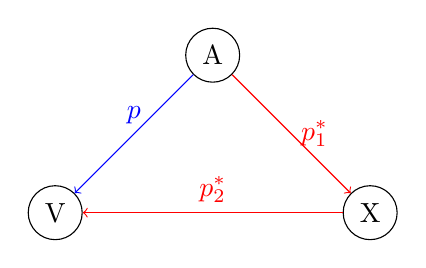
\begin{tikzpicture}
        % Nodi
        \node[circle, draw] (A) at (0,0) {A};
        \node[circle, draw] (V) at (-2,-2) {V};
        \node[circle, draw] (X) at (2, -2) {X};

    
        % Archi
        \draw[->, blue] (A) -- (V) node[midway, above] {$p$}; % Arco da A a B
        \draw[->, red] (A) -- (X) node[midway, right] {$p_1^*$}; % Arco da B a D
        \draw[->, red] (X) -- (V) node[midway, above] {$p_2^*$}; % Arco da D a C

    
    \end{tikzpicture}
\end{center}



\subsubsection{UCS con EXL}
Una prima forma di ottimizzazione della UCS la otteniamo introducendo una struttura dati detta \textit{Expansion List} o \textit{Lista delle Espansioni}
Questa lista è molto simile alla EQL, solo che in questo caso si aggiunge un nodo solo quando deve essere espanso, e non quando viene generato.



\subsection{Ricerca Informata}
Si parla di ricerca \textbf{non informata} quando dobbiamo affrontare un problema di Search avendo a disposizione \textbf{solo} 
il grafo e il criterio di scelta del prossimo nodo da esplorare.\\
Si parla, invece, di ricerca \textbf{informata} quando oltre alle informazioni precedenti abbiamo anche una stima $f(V)$ della bontà
del nodo $V$, ossia quanto è distante tale nodo dall'obiettivo. Tramite queste stime è possibile realizzare algoritmi con approccio
\textbf{Best-First} in cui il criterio di scelta di un nodo da esplorare avviene in base alla minimizzazione di $f(V)$.

\subsubsection{A*}
L'algoritmo A* è un algoritmo nato negli anni '60 per permettere al primo prototipo di Robot autonomo (Shakey) di arrivare da un punto
$A$ ad un punto $B$ col percorso più breve possibile. A* è praticamente identico a UCS, tranne per il fatto che il cost-to-go da ottimizzare è 
$f(s) = g(s) + h(s) $ dove $h(s)$ è detta \textbf{euristica di distanza} dall'ottimo. 
L'euristica dev'essere una funzione:
\begin{itemize}
    \item Computabile in tempo costante
    \item Ammissibile (ossia deve sottostimare il vero valore, o meglio la stima dev'essere ottimista)
\end{itemize} 
Trovare un'euristica sensata al problema, tuttavia, potrebbe non essere semplice.


